\documentclass[aspectratio=169,10pt]{beamer}

\usepackage[T1]{fontenc}
\IfFileExists{lmodern.sty}{\usepackage{lmodern}}{}
\usepackage{amsmath,amssymb,bm}
\usepackage{graphicx}
\usepackage{booktabs}
\usepackage{array}
\usepackage{animate}
\usepackage{tikz}
\usetikzlibrary{arrows.meta,positioning,shapes.geometric}
\usepackage{appendixnumberbeamer}
\newif\ifbackup
\backupfalse

\usetheme{default}
\usecolortheme{default}
\setbeamertemplate{navigation symbols}{}
\setbeamertemplate{itemize items}[circle]

\definecolor{ink}{HTML}{1B2430}
\definecolor{muted}{HTML}{6B7A8F}
\definecolor{accent}{HTML}{C4562F}
\definecolor{accentii}{HTML}{1F6F8B}
\definecolor{gold}{HTML}{D9A441}
\definecolor{softbg}{HTML}{EDEFF2}
\definecolor{rulegrey}{HTML}{C3C9D2}

\setbeamercolor{normal text}{fg=ink}
\setbeamercolor{frametitle}{fg=ink}
\setbeamercolor{title}{fg=ink}
\setbeamercolor{itemize item}{fg=accent}
\setbeamercolor{itemize subitem}{fg=accentii}
\setbeamercolor{structure}{fg=accent}
\setbeamercolor{alerted text}{fg=accent}

\setbeamerfont{frametitle}{size=\large,series=\bfseries}
\setbeamerfont{title}{size=\LARGE,series=\bfseries}
\setbeamerfont{footline}{size=\scriptsize}

\setbeamertemplate{frametitle}{%
  \vskip0.9ex%
  \begin{beamercolorbox}[wd=\paperwidth,leftskip=0.9cm,rightskip=0.9cm]{frametitle}%
    \usebeamerfont{frametitle}\insertframetitle%
    \\[0.5ex]{\color{accent}\rule{0.088\paperwidth}{1.3pt}}%
    {\color{rulegrey}\rule{0.795\paperwidth}{1.3pt}}%
  \end{beamercolorbox}%
  \vskip0.6ex%
}

\setbeamertemplate{footline}{%
  \hbox{%
    \begin{beamercolorbox}[wd=.80\paperwidth,ht=2.4ex,dp=1.4ex,leftskip=0.9cm]{}%
      {\color{muted}\scriptsize ASTG and the Earth Flyby Anomaly \quad$\cdot$\quad P.~A.~Nesvinga}%
    \end{beamercolorbox}%
    \begin{beamercolorbox}[wd=.20\paperwidth,ht=2.4ex,dp=1.4ex,rightskip=0.9cm]{}%
      \hfill{\color{muted}\scriptsize\insertframenumber}%
    \end{beamercolorbox}}%
  \vskip0pt%
}

\setbeamersize{text margin left=0.9cm,text margin right=0.9cm}

\newcommand{\ASTG}{ASTG}
\newcommand{\dVp}{\Delta V_p}
\newcommand{\dVinf}{\Delta V_\infty}
\newcommand{\Vp}{V_p}
\newcommand{\Vinf}{V_\infty}
\newcommand{\Dcosd}{\Delta\!\cos\delta}
\newcommand{\eps}{\varepsilon}
\newcommand{\sg}{s_g}
\newcommand{\kA}{\kappa_{\!\scriptscriptstyle A}}

\newcommand{\keybox}[1]{%
  \begin{center}\setlength{\fboxsep}{7pt}%
  \colorbox{softbg}{\parbox{0.90\textwidth}{\centering #1}}%
  \end{center}}

\newcommand{\figcap}[1]{{\footnotesize\color{muted} #1}}

\title{The Earth Flyby Anomaly in the Azimuthally\\[0.2ex]
       Symmetric Theory of Gravitation}
\author{P.~A.~Nesvinga}
\institute{Fundamental Theoretical Physics Group\\
           National University of Science \& Technology, Bulawayo}
\date{August 2026}

\begin{document}

{
\setbeamertemplate{footline}{}
\begin{frame}[plain]
  \vspace{0.45cm}
  \begin{center}
    {\color{accent}\rule{0.30\textwidth}{1.6pt}}\\[1.1em]
    {\usebeamerfont{title}\usebeamercolor[fg]{title}\inserttitle}\\[1.4em]
    {\large P.~A.~Nesvinga}\\[0.5em]
    {\color{muted}\normalsize Supervisors: Prof.~G.~G.~Nyambuya \quad$\cdot$\quad Prof.~B.~C.~Jones}\\[1.1em]
    {\footnotesize Fundamental Theoretical Physics Group\\
     Department of Applied Physics\\
     National University of Science \& Technology, Bulawayo}\\[1.3em]
    {\color{rulegrey}\rule{0.62\textwidth}{0.6pt}}\\[0.9em]
    {\footnotesize\itshape Presented in partial fulfilment of the requirements for the\\
     Master of Philosophy in Fundamental Theoretical Astrophysics}\\[1.0em]
    {\color{muted}\footnotesize August 2026}
  \end{center}
\end{frame}
}

\begin{frame}{Nine Earth flybys, four unexplained velocity increments}

  \begin{center}
    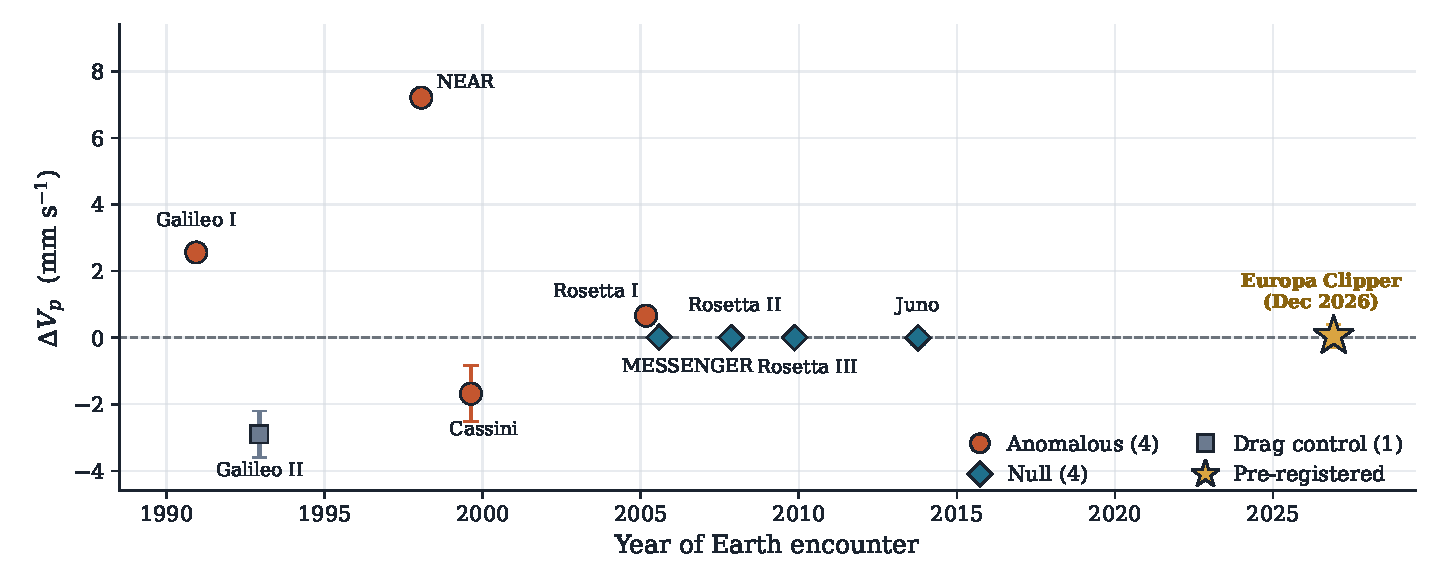
\includegraphics[width=0.86\textwidth]{figs/fig_timeline.pdf}
  \end{center}

  \vspace{-0.2em}
  \begin{columns}[T]
    \begin{column}{0.49\textwidth}
      \footnotesize
      Doppler tracking of gravity-assist encounters resolves the perigee
      speed to better than $10\,\mu$m\,s$^{-1}$ along track. Four
      encounters carry residuals of a few mm\,s$^{-1}$.
    \end{column}
    \begin{column}{0.49\textwidth}
      \footnotesize
      Anderson's empirical relation captures them,
      \[
        \frac{\dVinf}{\Vinf}=\kA\,\Dcosd,\qquad
        \kA=\frac{2\omega_\oplus R_\oplus}{c_0}=3.099\times10^{-6},
      \]
      with no derivation behind the constant.
    \end{column}
  \end{columns}

\end{frame}

\begin{frame}{A spinning body cannot have a spherical potential}

  \begin{columns}[T]
    \begin{column}{0.545\textwidth}
      \vspace{0.2em}
      Solving $\nabla^2\Phi=4\pi G\varrho$ for an azimuthally symmetric
      source, with $\Phi(r\to\infty)=0$ and Newton recovered at zeroth
      order:
      \[
        \Phi(r,\theta)=-\frac{GM_\star}{r}
        \left[1+\sum_{\ell=1}^{\infty}\lambda_\ell
        \Big(\frac{GM_\star}{rc_0^2}\Big)^{\!\ell}P_\ell(\cos\theta)\right]
      \]

      \footnotesize
      \vspace{0.3em}
      \begin{itemize}\setlength\itemsep{0.42em}
        \item $\lambda_\ell\equiv0$ when the source does not spin, so
              Newtonian gravity is recovered identically.
        \item $c_0$ enters through the structure of the
              Poisson--Laplace solutions, not through relativistic
              corrections: $\sg\equiv2GM_\oplus/c_0^2$ is the natural
              expansion length.
        \item At $\ell=1$ the correction is a $\cos\theta$ dipole about
              the spin axis: the north and south hemispheres sample
              different potentials at the same radius.
      \end{itemize}
    \end{column}
    \begin{column}{0.44\textwidth}
      \begin{center}
        \animategraphics[autoplay,loop,width=0.72\textwidth]{12}{anim/potential-}{0}{31}\\[0.3em]
        \figcap{Equipotentials deforming as the $\ell=1$ term switches
        on. Amplitude exaggerated for display.}
      \end{center}
    \end{column}
  \end{columns}

\end{frame}

\begin{frame}{Vis-viva evaluated where it is exact: at perigee}

  \begin{columns}[T]
    \begin{column}{0.47\textwidth}
      \footnotesize
      For hyperbolic excess speed $\Vinf$, energy conservation gives
      exactly
      \[
        v^2(r,\theta)=\Vinf^2+\frac{2GM_\oplus}{r}
        +\frac{2GM_\oplus \sg}{r^2}\lambda_1\cos\theta .
      \]

      \vspace{0.1em}
      At $r=r_p$ the velocity is purely tangential, $\dot r=0$, so
      $r_p^2v_p^2=GM_\oplus\ell$ holds with \emph{no} approximation.

      \vspace{0.5em}
      Differencing the inbound and outbound legs at that same radius
      cancels $\Vinf^2$ and the monopole identically:
      \[
        v_{p,\rm out}^2-v_{p,\rm in}^2
        =\frac{2GM_\oplus \sg\lambda_1}{r_p^2}
        \big(\cos\theta_{\rm out}-\cos\theta_{\rm in}\big).
      \]

      \vspace{0.4em}
      Everything flyby-specific drops out. What survives is the
      declination asymmetry of the trajectory.
    \end{column}
    \begin{column}{0.52\textwidth}
      \begin{center}
        \animategraphics[autoplay,loop,width=\textwidth]{12}{anim/flyby-}{0}{31}\\[0.2em]
        \figcap{NEAR sweeps $51^\circ$ of declination between its
        asymptotes, all of it south of the equator.}
      \end{center}
    \end{column}
  \end{columns}

\end{frame}

\begin{frame}{The \ASTG{} flyby formula}

  \keybox{$\displaystyle
    \frac{\dVp}{\Vp}=\frac{\lambda_1 \sg}{r_p(1+\eps)}\,\Dcosd
    =\frac{\lambda_1 \sg}{\ell}\,\Dcosd ,
    \qquad \ell\equiv r_p(1+\eps),\quad \sg=8.870\times10^{-3}\,\mathrm{m}$}

  \vspace{-0.35em}
  \begin{center}
    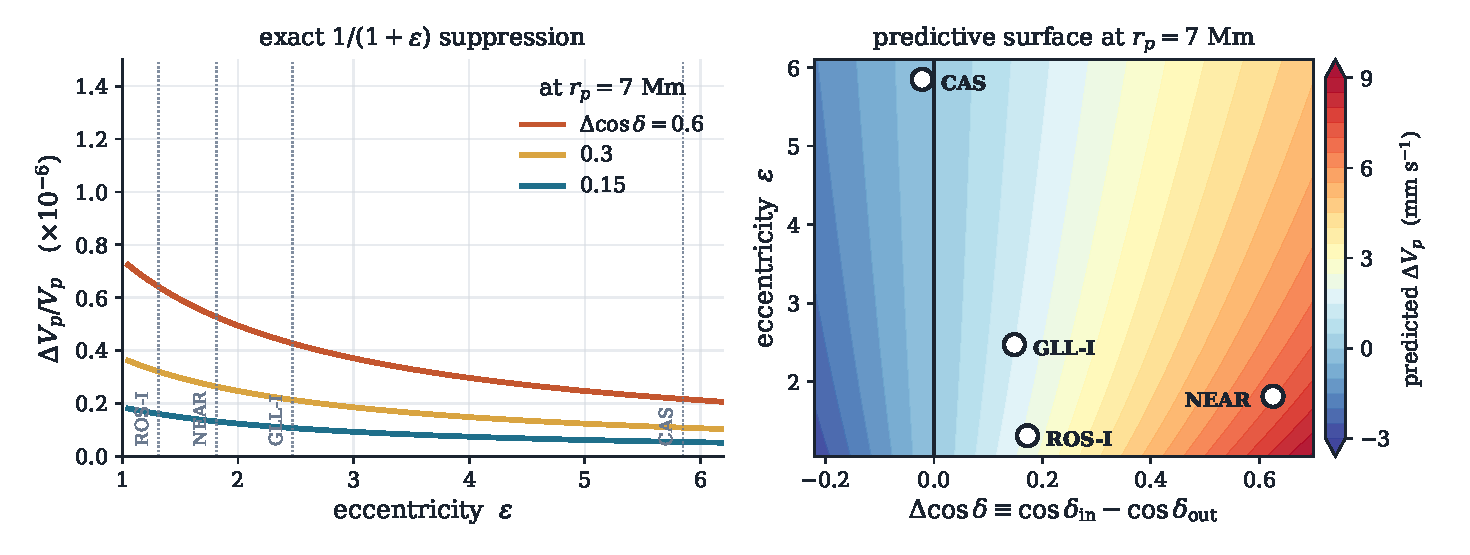
\includegraphics[width=0.845\textwidth]{figs/fig_formula.pdf}
  \end{center}

  \vspace{-0.45em}
  {\scriptsize
  $\lambda_1$ is one dimensionless property of the Earth, not a per-flyby
  parameter. Radial and eccentricity dependence are exact, and the
  intercept is zero by derivation.}

\end{frame}

\begin{frame}{The complete Earth-flyby inventory}

  \vspace{-0.2em}
  \begin{center}
  \footnotesize
  \renewcommand{\arraystretch}{1.12}
  \begin{tabular}{l c r r r r r r}
    \toprule
    Spacecraft & Date & $h_p$ & $\Vinf$ & $\dVp$ & $\eps$ &
    $\delta_{\rm in}$ & $\Dcosd$\\
    & & (km) & (km\,s$^{-1}$) & (mm\,s$^{-1}$) & & (deg) & \\
    \midrule
    \multicolumn{8}{l}{\color{accent}\itshape Anomalous}\\
    Galileo~I   & 1990-12-08 & 960  & 8.949  & $+2.560$ & 2.473 & $-12.52$ & $+0.1486$\\
    NEAR        & 1998-01-23 & 539  & 6.851  & $+7.210$ & 1.814 & $-20.76$ & $+0.6254$\\
    Cassini     & 1999-08-18 & 1171 & 16.010 & $-1.683$ & 5.850 & $-12.92$ & $-0.0215$\\
    Rosetta~I   & 2005-03-04 & 1955 & 3.863  & $+0.660$ & 1.312 & $-2.81$  & $+0.1726$\\
    \midrule
    \multicolumn{8}{l}{\color{accentii}\itshape Null}\\
    MESSENGER   & 2005-08-02 & 2347 & 4.056  & $+0.007$ & 1.360 & $+31.44$ & $+0.0044$\\
    Rosetta~II  & 2007-11-13 & 5295 & ---    & $\approx0$ & --- & $-10.84$ & $+0.034$\\
    Rosetta~III & 2009-11-13 & 2480 & ---    & $\approx0$ & --- & $+18.36$ & $+0.038$\\
    Juno        & 2013-10-09 & 561  & 9.831  & $<0.200$ & 2.681 & $+14.17$ & $+0.1980$\\
    \midrule
    Galileo~II  & 1992-12-08 & 303  & 8.877  & $-2.900$ & 2.319 & $-34.26$ & $-0.1699$\\
    \bottomrule
  \end{tabular}
  \end{center}

  \vspace{0.25em}
  {\scriptsize
  Anderson \textit{et al.} (2008); Jouannic \textit{et al.} (2015); Antreasian
  \& Guinn (1998). Declinations cross-checked against JPL Horizons state
  vectors, agreeing within $1\%$ for every flyby with published values.}

\end{frame}

\begin{frame}{One parameter, fitted globally, no intercept}

  \begin{columns}[T]
    \begin{column}{0.62\textwidth}
      \begin{center}
        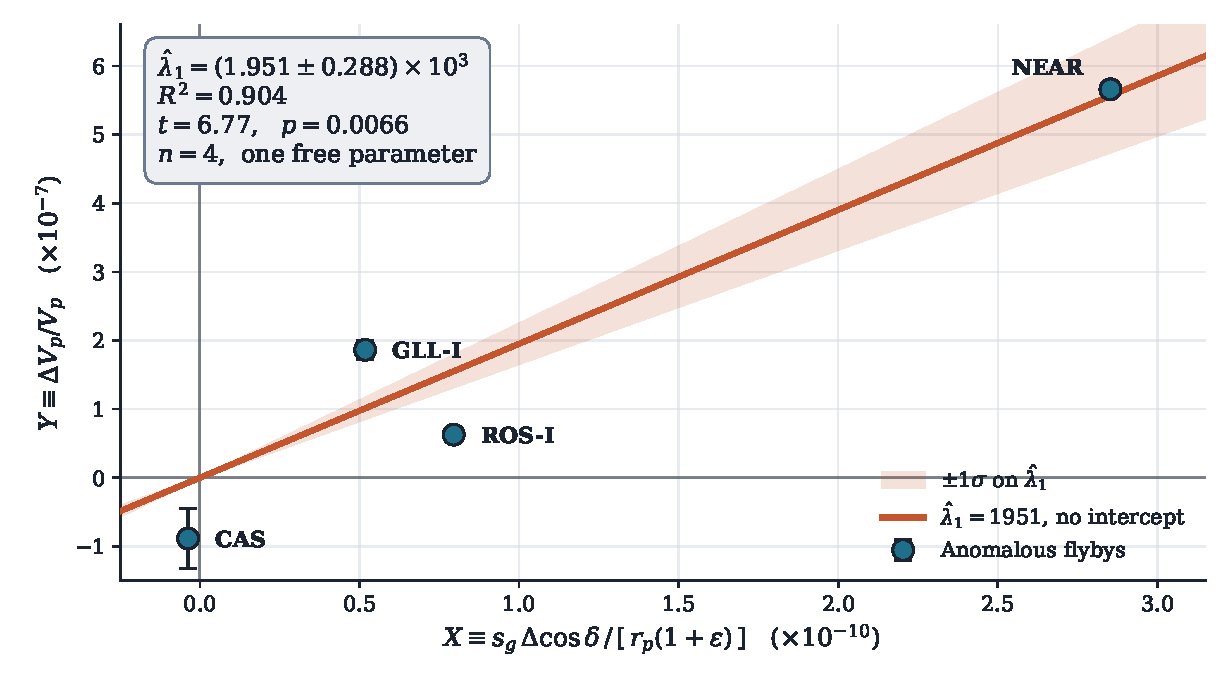
\includegraphics[width=\textwidth]{figs/fig_fit.pdf}
      \end{center}
    \end{column}
    \begin{column}{0.37\textwidth}
      \footnotesize
      \vspace{0.6em}
      Ordinary least squares on
      \[
        Y_i=\Big(\frac{\dVp}{\Vp}\Big)_i,\qquad
        X_i=\frac{\sg\,\Dcosd_i}{r_{p,i}(1+\eps_i)},
      \]
      so the fitted slope is $\lambda_1$ itself.

      \vspace{0.9em}
      \keybox{\footnotesize$\hat\lambda_1=(1.951\pm0.288)\times10^{3}$}

      \vspace{0.4em}
      The mixing-matrix construction of Nyambuya (2026), built from the
      fine-structure constant and Earth's spin angular momentum with no
      reference to flyby data at all, gives
      $\lambda_1\approx2.2\times10^{3}$.

      \vspace{0.5em}
      Two independent routes, agreeing to $\sim15\%$.
    \end{column}
  \end{columns}

\end{frame}

\begin{frame}{Predictions follow from geometry alone}

  \begin{center}
    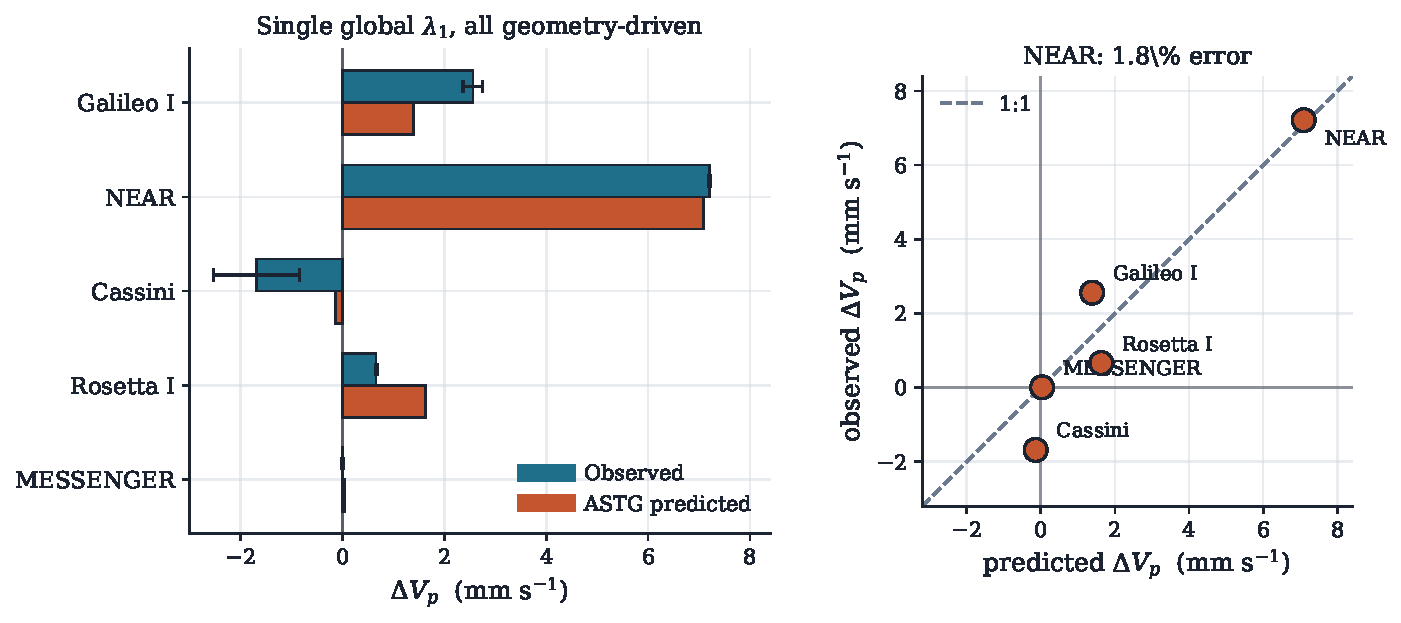
\includegraphics[width=0.90\textwidth]{figs/fig_predictions.pdf}
  \end{center}

  \vspace{-0.35em}
  {\scriptsize
  With $\hat\lambda_1$ fixed, each prediction follows from that flyby's own
  $r_p$, $\eps$ and $\Dcosd$. NEAR, the largest declination asymmetry in
  the record, is reproduced to $1.8\%$.}

\end{frame}

\begin{frame}{The fit does not rest on any single encounter}

  \begin{center}
    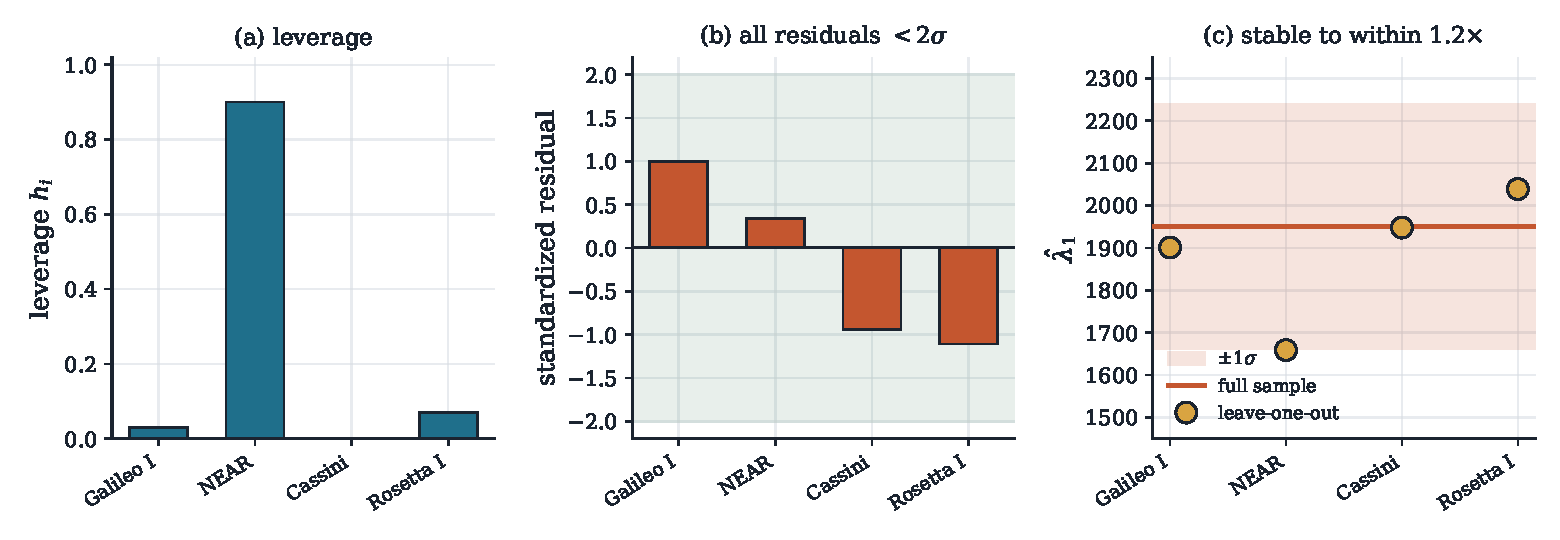
\includegraphics[width=0.96\textwidth]{figs/fig_diagnostics.pdf}
  \end{center}

  \vspace{0.2em}
  \begin{columns}[T]
    \begin{column}{0.49\textwidth}
      \footnotesize
      Refitting with each flyby removed in turn moves $\hat\lambda_1$
      between $1659$ and $2039$, every estimate within a factor $1.2$ of
      the full-sample value.
    \end{column}
    \begin{column}{0.49\textwidth}
      \footnotesize
      Leave-one-out prediction error, PRESS $=6.3$~(mm\,s$^{-1}$)$^2$,
      sits $34\%$ above the in-sample residual sum of squares
      $4.7$~(mm\,s$^{-1}$)$^2$.
    \end{column}
  \end{columns}

\end{frame}

\begin{frame}{A regularity in the record: hemisphere sorts the sample}

  \begin{center}
    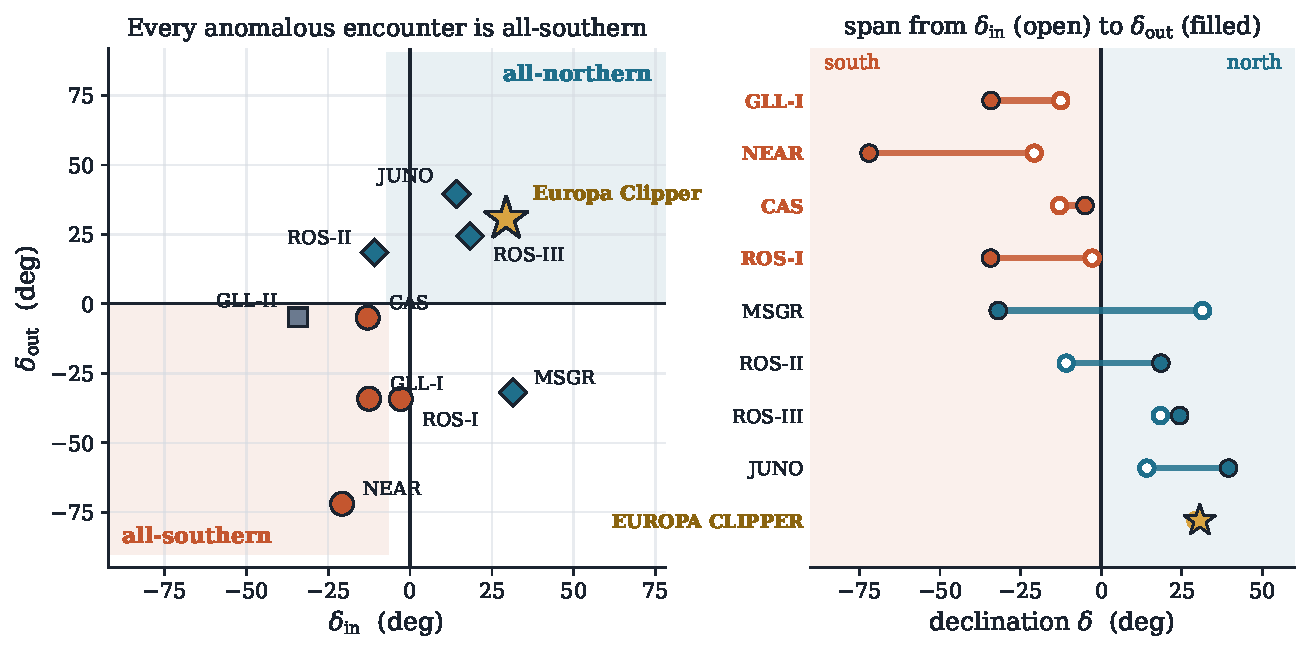
\includegraphics[width=0.855\textwidth]{figs/fig_hemisphere.pdf}
  \end{center}

  \vspace{-0.45em}
  {\scriptsize
  All four anomalous flybys are all-southern. Both all-northern
  encounters, \textit{Rosetta}~III and \textit{Juno}, are null. The
  pattern was found in the data rather than built into the model, which
  is what makes the next encounter a test of it.}

\end{frame}

\begin{frame}{A pre-registered test: \textit{Europa Clipper}, December 2026}

  \begin{columns}[T]
    \begin{column}{0.485\textwidth}
      \vspace{0.1em}
      \begin{center}
        \animategraphics[autoplay,loop,width=\textwidth]{12}{anim/europa-}{0}{31}
      \end{center}
      \vspace{-0.1em}
      \figcap{JPL Horizons solution queried 2026 August 6, incorporating
      tracking through July 20. Inbound and outbound legs agree on
      $\Vinf$ to $0.5$~m\,s$^{-1}$.}
    \end{column}
    \begin{column}{0.495\textwidth}
      \begin{center}
        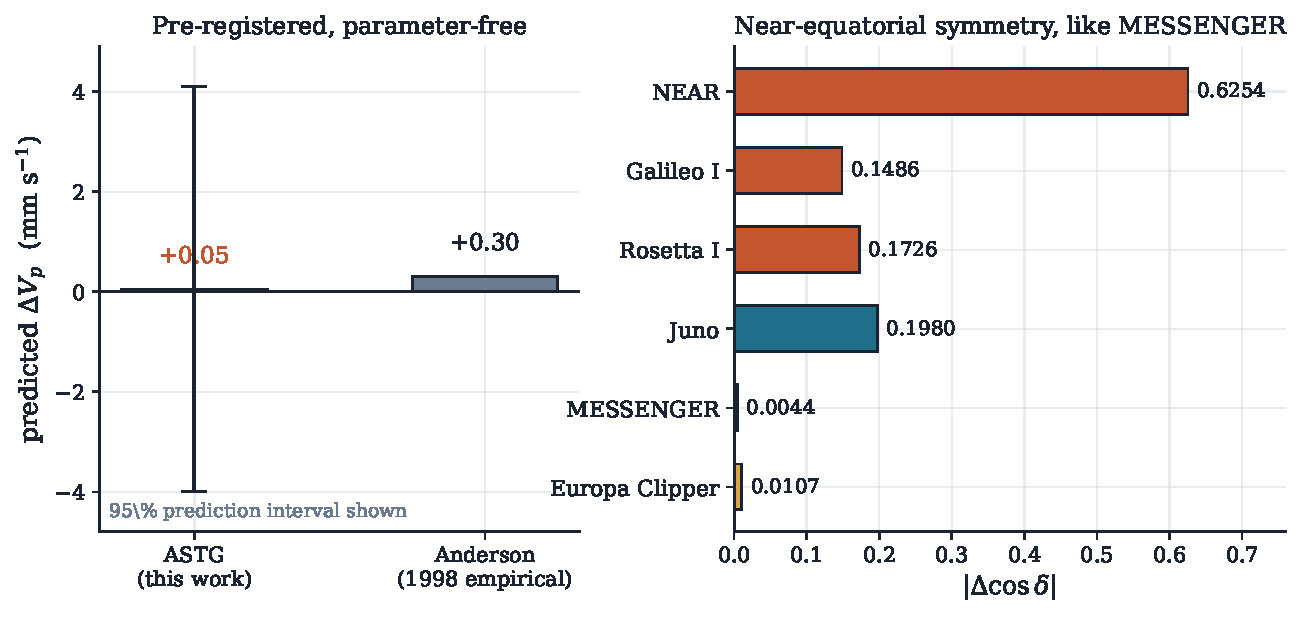
\includegraphics[width=\textwidth]{figs/fig_europa.pdf}
      \end{center}
      \vspace{-0.2em}
      \footnotesize
      Closest approach 2026 December 3, 20:15:21 TDB, at
      $r_p=9.606$~Mm and $\Vinf=11.558$~km\,s$^{-1}$, giving
      $\eps=4.219$ and $\Dcosd=+0.0107$.

      \vspace{0.35em}
      The prediction is fixed before the encounter, with $\hat\lambda_1$
      carried over unchanged from the 1990--2005 sample. Nothing is
      adjustable.
    \end{column}
  \end{columns}

\end{frame}

\begin{frame}{Where the work stands}

  \vspace{-0.1em}
  \begin{center}
  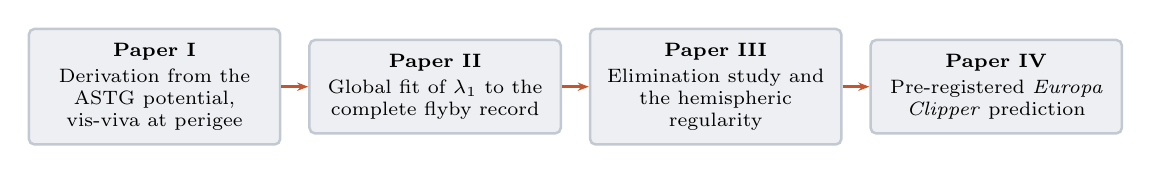
\begin{tikzpicture}[
      node distance=0.34cm,
      pbox/.style={draw=rulegrey,line width=0.9pt,fill=softbg,rounded corners=2pt,
                   text width=2.84cm,align=flush center,inner sep=5pt,
                   font=\scriptsize},
      lbl/.style={font=\scriptsize\bfseries,color=accent}]
    \node[pbox] (p1) {\textbf{Paper I}\\[0.2em] Derivation from the \ASTG{}
      potential, vis-viva at perigee};
    \node[pbox,right=of p1] (p2) {\textbf{Paper II}\\[0.2em] Global fit of
      $\lambda_1$ to the complete flyby record};
    \node[pbox,right=of p2] (p3) {\textbf{Paper III}\\[0.2em] Elimination
      study and the hemispheric regularity};
    \node[pbox,right=of p3] (p4) {\textbf{Paper IV}\\[0.2em] Pre-registered
      \textit{Europa Clipper} prediction};
    \draw[-{Stealth[length=4pt]},color=accent,line width=0.9pt] (p1)--(p2);
    \draw[-{Stealth[length=4pt]},color=accent,line width=0.9pt] (p2)--(p3);
    \draw[-{Stealth[length=4pt]},color=accent,line width=0.9pt] (p3)--(p4);
  \end{tikzpicture}
  \end{center}

  \vspace{0.3em}
  \begin{columns}[T]
    \begin{column}{0.485\textwidth}
      \footnotesize
      \textbf{Established}
      \begin{itemize}\setlength\itemsep{0.30em}
        \item A closed-form flyby anomaly derived from a gravitational
              potential, with one mission-independent constant and exact
              radial and eccentricity dependence.
        \item $\hat\lambda_1=(1.951\pm0.288)\times10^{3}$ from the
              complete anomalous sample, $R^2=0.904$, $p=0.0066$.
        \item Independent agreement to $\sim15\%$ with a coupling
              derived from $\alpha_0$ and Earth's spin alone.
      \end{itemize}
    \end{column}
    \begin{column}{0.485\textwidth}
      \footnotesize
      \textbf{In progress}
      \begin{itemize}\setlength\itemsep{0.30em}
        \item Reconstruction of the \textit{Europa Clipper} encounter
              against the pre-registered $+0.05$~mm\,s$^{-1}$.
        \item Extension to Jupiter and Saturn encounters, where
              $\lambda_1$ is set by that body's own spin multipoles
              (JUICE, Ulysses).
        \item The $\varphi$-dependent coupling, integrated exactly to
              $O(\hat k)$, against the full record.
      \end{itemize}
    \end{column}
  \end{columns}

  \vspace{0.6em}
  {\scriptsize\color{muted}
  Code and data: \texttt{github.com/cerealrose}}

\end{frame}

\ifbackup
\appendix

\begin{frame}{Backup: sample size and leverage}
  \footnotesize
  Four anomalous encounters is the complete population of Earth gravity
  assists with published Doppler residuals, not a subsample. In the
  no-intercept regression the leverage $h_i=X_i^2/\sum_j X_j^2$ places
  $0.90$ on NEAR, whose large $\Dcosd$ coincides with a small
  $r_p(1+\eps)$. Cassini contributes $h\approx2\times10^{-4}$: its
  near-null $\Dcosd$ suppresses both its weight and its information
  content.

  \vspace{0.5em}
  Dropping NEAR moves $\hat\lambda_1$ by $-15\%$, the largest of the
  four; dropping Cassini moves it by $-0.2\%$. Cook's $D=1.03$ for NEAR
  sits above the conventional $4/n$ guideline, though at $n=4$ that
  threshold is illustrative rather than decisive. The substantive
  statement is the leave-one-out spread: a factor of $1.2$.
\end{frame}

\begin{frame}{Backup: the \textit{Juno} encounter}
  \footnotesize
  \textit{Juno} 2013 has $\Dcosd=+0.198$ and a reconstructed anomaly
  below $0.200$~mm\,s$^{-1}$, against a point prediction of
  $+1.95$~mm\,s$^{-1}$. Paper~III uses that gap to eliminate eight
  candidate resolutions rather than to absorb it.

  \vspace{0.4em}
  \begin{itemize}\setlength\itemsep{0.20em}
    \item Spacecraft spin, atmospheric drag, general-relativistic and
          classical perturbations, and the $\ell=2$ multipole: short by
          two to eleven orders of magnitude.
    \item Gravity-model fidelity: excluded by independent reprocessing
          of the tracking data.
    \item Thermal recoil of the $60$~m$^2$ solar array through the only
          eclipse of cruise: bounded at $0.077$~mm\,s$^{-1}$, a factor
          of $25$ short.
    \item The $\varphi$-dependent coupling fitted to the anomalous
          sample raises the prediction to $+2.37$~mm\,s$^{-1}$; the
          literal $\ell=1$ colatitude term $\Delta\!\sin\delta$ enters
          with $\hat\lambda_b/\hat\lambda_a=1.1\times10^{-3}$,
          consistent with zero.
  \end{itemize}

  \vspace{0.3em}
  What survives is the hemispheric regularity, which
  \textit{Europa Clipper} tests.
\end{frame}

\begin{frame}{Backup: per-flyby coupling}
  \footnotesize
  Inverting the formula flyby by flyby gives
  $\lambda_1^{(i)}\times10^{-3}$ of $3.60$ (Galileo~I), $1.98$ (NEAR),
  $23.93$ (Cassini) and $0.79$ (Rosetta~I).

  \vspace{0.4em}
  Cassini's propagated uncertainty is
  $\sigma_{\lambda_1}\approx12.0\times10^{3}$, comparable to its own
  central value, so its formal deviation from the global fit is
  $\sim1.8\sigma$: its near-null $\Dcosd$ sits in the denominator.
  Galileo~I and Rosetta~I carry small propagated uncertainties, so their
  spread reflects flyby-to-flyby physical scatter rather than
  measurement error in $\dVp$.

  \vspace{0.4em}
  The global fit is the falsifiable object; $\lambda_1^{(i)}$ is
  diagnostic. Identifying the physical variable behind the
  Galileo~I / Rosetta~I offset is the open question the
  $\varphi$-dependent coupling is aimed at.
\end{frame}
\fi

\end{document}
